The large scale structure of our local universe is dominated by voids and filamentary structures of groups and clusters of galaxies 
(e.g., Courtois et al.\ 2013).  Half of the Local Volume galaxies reside in loose groups and associations, such as the Sculptor filament and the Canes Venatici Cloud (Karachenstev 2005). The nearest such structure is the NGC~3109 association (see Figure 1), an association of 5 dwarf galaxies in Leo, Sextans, and Antlia (van den Bergh 1999; Tully et al.\ 2006). This galaxy association, with a linear extent of 1.2~Mpc across the sky (Bellazzini et al.\ 2013), lies just at the edge of the Local Group, at a distance of 1.3--1.7 Mpc. It is  presumably on its first infall towards the Local Group, thus having still retained its filamentary structure. 


The newest member of the NGC~3109 association, Leo P, was recently discovered as part of a blind H~I survey;
it has an H~I mass of $10^6$ solar masses and a stellar mass about $3\times10^5$~M$_{\odot}$, and is extremely metal-poor (Giovanelli et al.\ 2013).
This suggests to us that additional  faint members of the group may await discovery. Tidal debris from interactions between group members may also be located along the filament; indeed tidal substructure near the Antlia dwarf suggestive of an interaction with NGC~3109 was recently discovered by Penny et al.\ (2012). Completing the substructure census and probing the faintest end of the luminosity function in the nearest filamentary structure are the goals of this proposal. Detected low-surface brightness structures will be characterized in terms of structural properties and their association to the sub-group will be pursued via follow-up tip-of-the-red-giant-branch (TRGB; Lee et al.\ 1993) measurements. Filamentary structures are considered to be in an earlier stage of their evolution, thus a complete characterization of the interacting environment of the NGC~3109 structure will provide us with insights to lend interpretation to more distant structures, such as the Sculptor filament (e.g. Jerjen et al.\ 1998).

Using LBT imaging of Leo~P, McQuinn et al.\ (2013) measured the TRGB magnitude in this galaxy to be $i=22.1$. 
This is a useful guide to the kind of depth needed to uncover the distant and sparsely populated dwarfs which
might be undiscovered in the NGC 3109 filament. While the region is covered by existing  and planned
survey data, none are deep enough to detect the anticipated faint structures.
The northern portion of  the filament, from Leo P to  Sextans B, is covered in the SDSS imaging, but 
while the SDSS  depth ($g=22.2$, $i=21.3$) is adequate for the discovery and characterization of nearby faint dwarfs
within the virial radius of the Milky Way (e.g., Koposov et al.\ 2008), it is inadequate to  dwarfs such as Leo~P . 
The southern portion of the filament does not have currently useful survey data:
the VST/KiDS survey just misses  the region between Sextans A and B, and the VST/ATLAS survey is
only of SDSS depth,  thus unsuitable for our study. The SkyMapper southern sky survey (Keller et al.\ 2007) is planned 
to cover the southern sky to slightly greater than SDSS depth, but it is unclear when those data might become available
or what their eventual depth will be.

A dedicated survey using a 4-m class telescope is required to detect low-luminosity galaxies at the distance of the NGC~3109 filament and 
we propose a survey  of this nearest filamentary structure with CFHT/MegaCam. MegaCam's ability to go both wide and deep is essential for this project: the nearby nature of the filament means that it covers a large area of sky, and faint dwarf galaxies are resolved into individual stars.
Mapping the NGC~3109 filament will lead to a measurement of the galaxy luminosity function and interaction history to extremely faint
levels in a `primitive' galaxy structure, with implications for cosmological models of galaxy formation and evolution.



%Bellazzini, M. et al.  2013, A\&A 559, L11\\
%Chiboucas, K. et al.\  2009, AJ, 137, 3009\\
%Courtois, H.R. et al.\ 2013, AJ, 146, 69\\
%Giovanelli, R. et al.\ 2013, AJ, 146, 15\\
%Jerjen, H. et al.\ 1998, AJ, 116, 2873\\
%Karachentsev, I. 2005, AJ, 129, 178 \\
%Keller, S.C. et al.\ 2007, PASA, 24, 1\\
%Koposov, S. et al.\ 2008, ApJ, 686, 279\\
%Lee, M.G et al.\ 1993, ApJ, 417, 993\\ 
%McQuinn, K.B.W. et al. 2013, AJ, 146, 145\\
%Penny, S.J. et al. 2012, ApJ, 758, L32\\
%Tully, R.B. et al.\ 2006, AJ, 132, 729\\
%van den Bergh, S. 1999, ApJ, 517, L97\\

\clearpage


% get these ordered correctly at end
\section*{References}

\begin{table}[h]
\begin{tabular}{ll}
Bellazzini, M. et al.\  2013, A\&A 559, L11 & Pawlowski, M.S. \&  McGaugh, S.S. 2014, MNRAS, 440, 908\\
Bellazzini, M. et al.\  2014, A\&A 566, 44 & Koposov, S. et al.\ 2008, ApJ, 686, 279\\
Chiboucas, K. et al.\  2009, AJ, 137, 3009 & Lee, M.G. et al.\ 1993, ApJ, 417, 993\\
Courtois, H.R. et al.\ 2013, AJ, 146, 69 &  McQuinn, K.B.W. et al. 2013, AJ, 146, 145\\
Giovanelli, R. et al.\ 2013, AJ, 146, 15 & Penny, S.J. et al. 2012, ApJ, 758, L32\\
Jerjen, H. et al.\ 1998, AJ, 116, 2873  &  Tully, R.B. et al.\ 2006, AJ, 132, 729\\
Karachentsev, I. 2005, AJ, 129, 178 &van den Bergh, S. 1999, ApJ, 517, L97\\
Keller, S.C. et al.\ 2007, PASA, 24, 1\\
\end{tabular}
\end{table}



\begin{figure}
%\caption{The NGC 3109 association shown in Cartesian coordinates centred on NGC 3109. From Bellazzini et al.\ (2013).}
%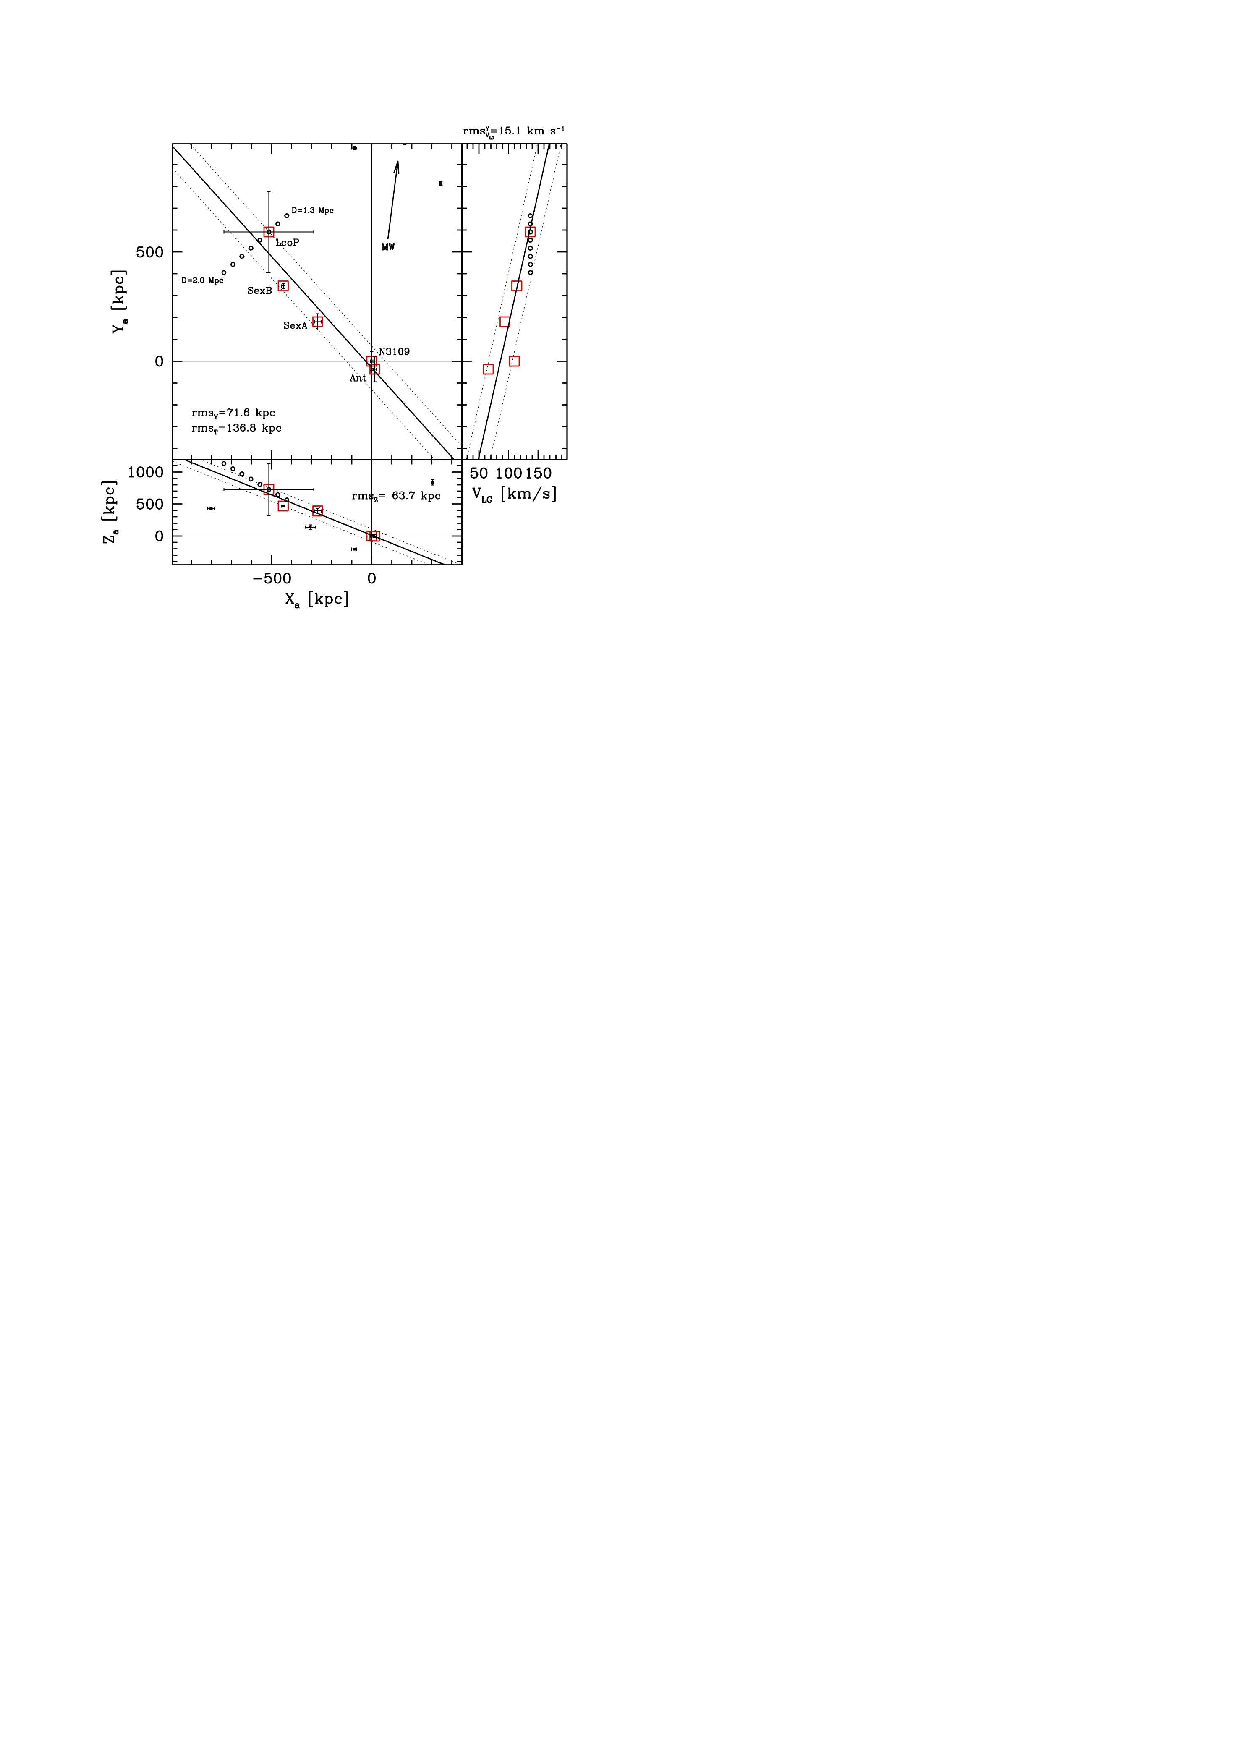
\includegraphics[scale=1.2]{bellaz_fig1}
\caption{Equatorial coordinates of the NGC 3109 association galaxies. The present proposal is to image
a 1-degree-wide strip from Sextans A to Leo P using MegaCam.}
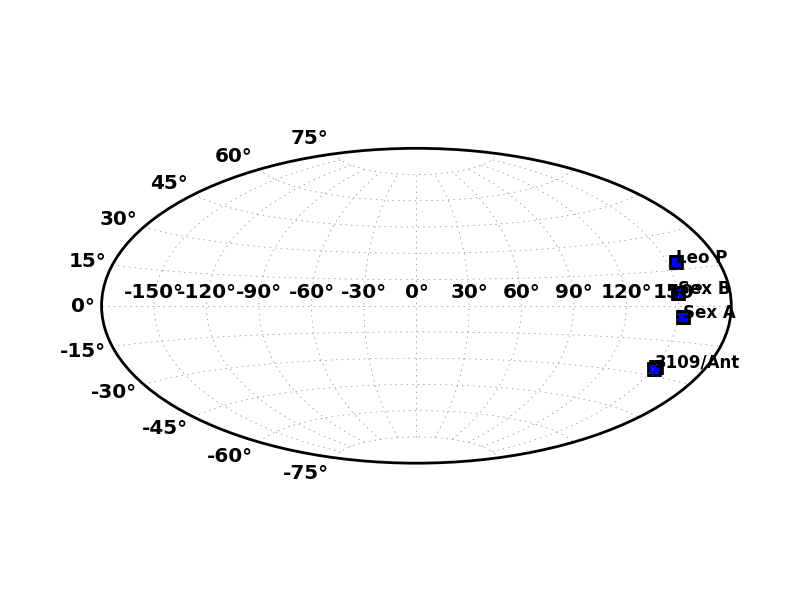
\includegraphics[scale=0.7]{n3109_group_sky}

\end{figure}


